% Finished July 18, 2013
% Put into format of VUW Thesis on March 20, 2014.
% Cut out of Chapter 6 and formed into Appendix D on Friday, 21 March 2014.

\documentclass[12pt, a4paper, twoside, openright]{book}

\usepackage{vuwthesis} % sets up some local things, mostly the front page

\setlength{\intextsep}{12pt} % set space above and below in-line float
\setlength{\abovecaptionskip}{0pt} % set space between figure and caption.


\usepackage{amssymb, amsmath}
%\usepackage{mathtools}
\usepackage{tikz}
\usetikzlibrary{calc}

\newcommand{\beff}{\ensuremath{b_{\mathrm{eff}}}}
\newcommand{\bhom}{\ensuremath{b_{\mathrm{hom}}}}

%\usepackage{marvosym}

\usepackage{etoolbox}
\newtoggle{compilealone}
\toggletrue{compilealone}

\title{Appendix D: The Variational Formulation}
\author{Nat Lund}

\begin{document}
\chapter{The Variational Formulation}\label{C:variational}

In this appendix, we provide an in-depth explanation of the variational formulation of PDEs and its relation to the calculus of variations.  This appendix is intended to be a stand-alone document, that can be read without reference to Chapter 6.  As such, it contains material which is duplicated in Chapter 6.

\clearpage
\section{Variational Form}

The variational form comes originally from the Calculus of Variations.  The canonical use for the calculus of variations is with a \emph{minimization} problem.  We seek a \emph{function} on a domain that minimizes some quantity.  The quantity to be minimized is a \emph{functional}, a mapping from the space of functions to the real numbers.  The functional will be some kind of integral, with the integrand being some combination of the function, its derivatives (of various order), and position in the domain.

\begin{equation}
F(u) = \int_a^b f(u,u', ...\, ,x) \; dx,  \qquad F(u) \mapsto \mathbb{R}
\end{equation} 

The boundary values of the function $u(x)$ are given.  The basic concept of calculus of variations is to take $u(x)$ to be the solution function that minimizes the functional $F$.  That being the case, any \emph{variation} away from $u$, however small, will increase $F$.  Let $v(x)$ be an arbitrary function that is zero at the boundary (i.e. zero at $a$ and $b$), and let $\epsilon$ be a small parameter. Then:
\begin{equation}
F(u) \leq F(u + \epsilon v) \qquad \forall v: v(a) = v(b) = 0
\end{equation}
This minimizing function and variation are depicted in Figure (\ref{variation}).

\begin{figure}[ht]
\centering
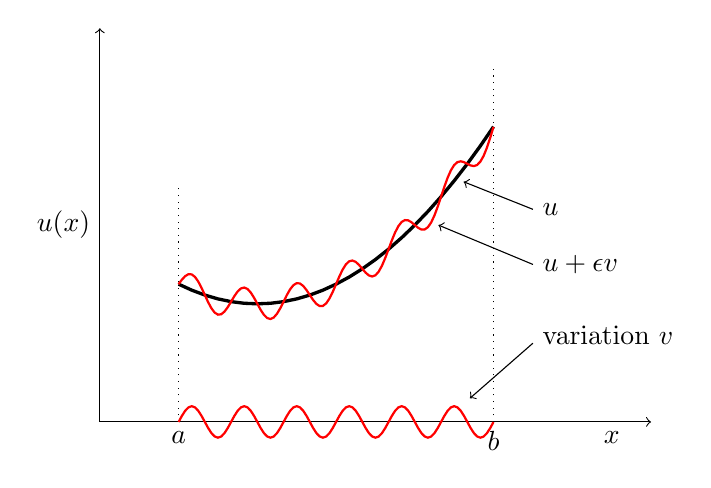
\begin{tikzpicture}

\draw[<->] (7,0) -- (0,0) -- node[left]{$u(x)$} (0,5);
\node at (6.5,0) [below] {$x$};
\draw[dotted] (1,0) -- +(0,3);
\draw[dotted] (5,0) -- +(0,4.5);
\node at (1,0)[below] {$a$};
\node at (5,0)[below] {$b$};

%\draw[very thick] (1,2) to [out=-50, in=180] (2,1.5) to [out=0,in=240] (5,3.5);
\draw[very thick, domain=1:5] plot (\x, { 1.5 + 0.25*(\x-2)*(\x-2) });
\draw[color=red,thick, samples=97, domain=1:5] plot (\x, { 0.2 * sin( 3*pi*(\x-1) r) } );
\draw[color=red,thick, samples=97, domain=1:5] plot (\x, { 1.5 + 0.25*(\x-2)*(\x-2) + 0.2 * sin( 3*pi*(\x-1) r)  });

\draw[<-](4.7,0.3) -- (5.5,1);
\node at (5.5,1.1)[right] {variation $v$};
\draw[<-] (4.62,3.05) -- (5.5,2.7);
\node at (5.5,2.7)[right] {$u$};
\draw[<-] (4.3,2.5) -- (5.5,2);
\node at (5.5,2)[right] {$u + \epsilon v$};

\end{tikzpicture}
\caption{The minimizing function $u(x)$ and an arbitrary variation $v(x)$ added to it.}\label{variation}
\end{figure}

For an arbitrary variation $v$, the small parameter $\epsilon$ can be treated as a variable, so that $F(u + \epsilon v)$ is a function from $\mathbb{R}$ to $\mathbb{R}$. Since $u$ minimizes $F$, $\epsilon = 0$ minimizes $F(\epsilon): \mathbb{R} \mapsto \mathbb{R}$. % Here's the cunning bit: 
The minimum is a stationary point, so the \emph{slope} of $F(\epsilon)$ is zero also at the minimum.  That is, for minimizing function $u$, for any variation $v$,

\begin{equation}
\frac{d}{d \epsilon} F(u + \epsilon v) = 0
\end{equation}
This is shown in Figure (\ref{minimum}).

\begin{figure}[ht]
\centering
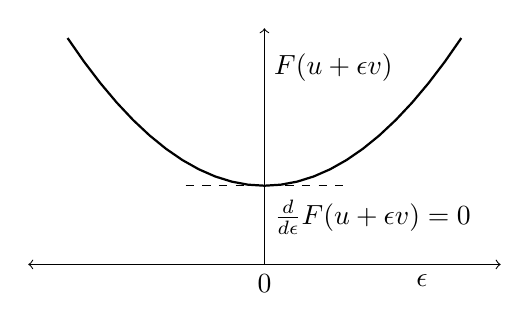
\begin{tikzpicture}
\draw[<->] ( -3,0) -- (3,0);
\draw[->] (0,0) --  (0,3);
\node at (2,0) [below] {$\epsilon$};
\node at (0,0) [below] {0};
\node at (0,2.5)[right]{$F(u + \epsilon v) $};

%\draw[thick,dashed] (-2.5,3) to [out=-60, in=180] (0,1) to [out=0, in=240] (2.5,3);
\draw[thick, domain=-2.5:2.5] plot ( \x, {1 + 0.3* \x*\x} );

\draw[dashed] (-1,1) -- +(2,0);
\node at (0,0.6) [right] {$\frac{d}{d \epsilon} F(u + \epsilon v) = 0$};
 
\end{tikzpicture}
\caption{The slope of $F(\epsilon)$ is zero at the minimum of $F(\epsilon)$.}\label{minimum}
\end{figure}


\subsection{Example: Energy Balance}

For example, consider a film of soapy water suspended across an aperture.  At equilibrium, the soap film lies in the $x,y$ plane.  Let $u(x,y)$ be the the height of the film above the $x,y$ plane (at point ($x,y$)), as in the schematic of Figure (\ref{soapy}).

\begin{figure}[ht]
\centering
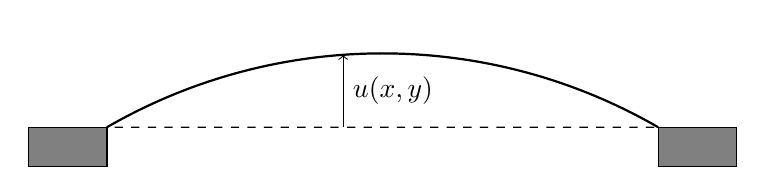
\begin{tikzpicture}

\draw [thick] (0,0) arc (120:60:7cm);
\draw (0,0) arc (120:60:7cm) [dashed] -- (0,0);

\draw [fill=gray] (0,0) rectangle ++(-1,-0.5);
\draw [fill=gray] (7,0) rectangle ++(1,-0.5);

\draw[->] (3,0) -- node[right]{$u(x,y)$} ++(0,0.92);

\end{tikzpicture}
\caption{A film of soapy water suspended across an aperture.}\label{soapy}
\end{figure}

Assume some force below the film distorts it, pushing it upwards.  The force does work on the soap film. If $f$ is the force on the film per unit area (pressure), then the work done moving an infinitesimal area element $dA$ a distance $u(x,y)$ is $dW = u f dA$. Thus the total work done on the soap film is the integral: 
\begin{equation}
W = \int_{\Omega} f u \,dA
\end{equation} 
The geometry of the work done appears in Figure (\ref{work}).
\begin{figure}[ht]
\centering
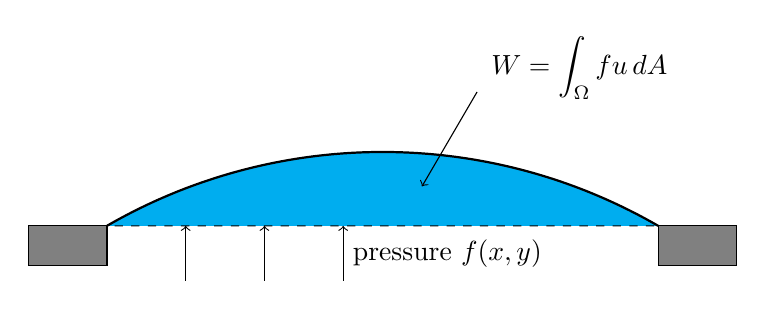
\begin{tikzpicture}

\draw [fill=cyan] (0,0) arc (120:60:7cm) [dashed] -- (0,0);
\draw [thick] (0,0) arc (120:60:7cm);

\draw [fill=gray] (0,0) rectangle ++(-1,-0.5);
\draw [fill=gray] (7,0) rectangle ++(1,-0.5);

\draw[<-] (3,0) -- node[right]{pressure $f(x,y)$} ++(0,-0.7);
\draw[<-] (1,0) -- ++(0,-0.7);
\draw[<-] (2,0) -- ++(0,-0.7);

\draw[<-] (4,0.5) -- ++(0.7,1.2);
\node at (6,2) {$\displaystyle W = \int_{\Omega} f u \,dA $};
\end{tikzpicture}
\caption{The work done by the pressure distorting the soap film.}\label{work}
\end{figure}


The work done on the soap film is stored as elastic potential energy.  The soap film has a surface tension that acts tangentially to the surface.  A virtual length $dy$ has a force $2 \gamma dy$ acting perpendicularly to it. The force is \emph{constant,} so if the length is moved distance $dx$, creating new area $dxdy$, the work done is $ 2 \gamma dxdy$.  Thus, the change in potential energy is proportional to the change in area.

Consider a tangent plane of $u(x,y)$ located above an infinitesimal area element $dxdy$.  The tangent plane is bounded by the vectors $(dx,0,dx \partial_x u)$ and $(0,dy,dy \partial_y u)$. Their cross product is the normal vector to the plane\\
 $\vec{n} = (-dxdy \partial_x u, -dxdy \partial_y u, dxdy) $. The area of the infinitesimal tangent plane is equal to the magnitude of the normal vector:
\begin{equation}
dA = |\vec{n}| = dxdy \sqrt{1 + \partial_x u^2 + \partial_y u^2}
\end{equation}
For convenience, we use $|\nabla u|^2 = \nabla u \cdot \nabla u = \partial_x u^2 + \partial_y u^2  $.  The total area of the soap film is:
\begin{equation}
A =  \int_{\Omega} \sqrt{1 + |\nabla u|^2} \;dxdy
\end{equation}

\clearpage
If the soap bubble is distorted not too far from its equilibrium shape, then $\partial_x u \ll 1$ and $\partial_y u \ll 1$, so that:
\begin{equation}
\sqrt{1 + |\nabla u|^2} \approx \sqrt{1 + |\nabla u|^2 + \frac{1}{4} |\nabla u|^4}
= \sqrt{(1 + \frac{1}{2} |\nabla u|^2)^2}
= 1 + \frac{1}{2} |\nabla u|^2
\end{equation}
Then the \emph{change} in area from the equilibrium area is:
\begin{equation}
\int_{\Omega} 1 + \frac{1}{2} |\nabla u|^2 \;dxdy - \int_{\Omega} dxdy = 
\int_{\Omega} \frac{1}{2} |\nabla u|^2 \;dxdy
\end{equation}
Let $k$ be the surface tension coefficient.  Then the elastic potential energy is:
\begin{equation}
U = k \frac{1}{2} \int_{\Omega}  |\nabla u|^2 \;dA 
\end{equation} 
This shown in the schematic of Figure (\ref{potential}).

\begin{figure}[ht]
\centering
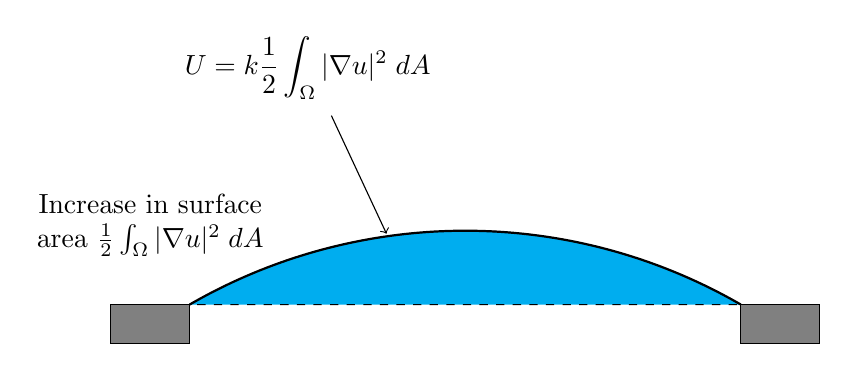
\begin{tikzpicture}

\draw [fill=cyan] (0,0) arc (120:60:7cm) [dashed] -- (0,0);
\draw [thick] (0,0) arc (120:60:7cm);

\draw [fill=gray] (0,0) rectangle ++(-1,-0.5);
\draw [fill=gray] (7,0) rectangle ++(1,-0.5);

%\draw[<-] (3,0) -- node[right]{pressure $f(x,y)$} ++(0,-0.7);
%\draw[<-] (1,0) -- ++(0,-0.7);
%\draw[<-] (2,0) -- ++(0,-0.7);

%\draw[<-] (4,0.5) -- ++(0.8,2.2);
%\node at (6,3) {$\displaystyle W = \int_{\Omega} f u \,dA $};

\draw[<-] (2.5,0.9) -- ++(-0.7,1.5);
\node at (1.5,3) {$\displaystyle U = k \frac{1}{2} \int_{\Omega}  |\nabla u|^2 \;dA  $};

\renewcommand{\baselinestretch}{1.00}
\node at (-0.5,1)[align=center] {Increase in surface\\ area $ \frac{1}{2} \int_{\Omega}  |\nabla u|^2 \;dA $ };

\end{tikzpicture}
\caption{The elastic potential energy due to the increase in area of the soap film.}\label{potential}
\end{figure}

\clearpage
The elastic potential energy is exactly equal to the work done on the soap film by the pressure:
\begin{equation}
k \frac{1}{2} \int_{\Omega} |\nabla u|^2 \;dA = \int_{\Omega} f u \;dA
\end{equation}
A summary schematic is shown in Figure (\ref{balance}).

\begin{figure}[ht]
\centering
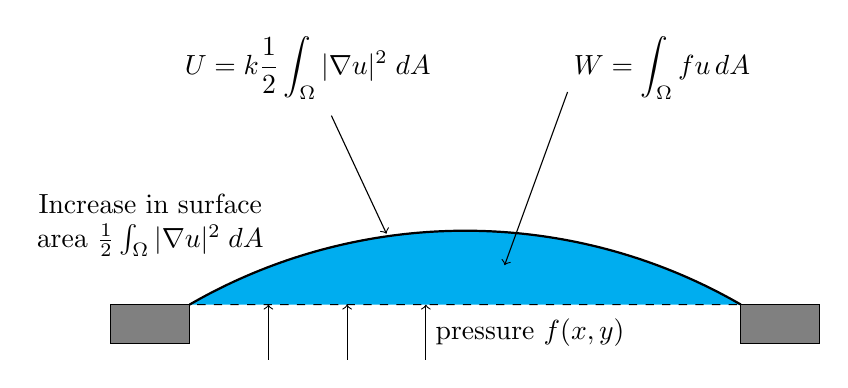
\begin{tikzpicture}

\draw [fill=cyan] (0,0) arc (120:60:7cm) [dashed] -- (0,0);
\draw [thick] (0,0) arc (120:60:7cm);

\draw [fill=gray] (0,0) rectangle ++(-1,-0.5);
\draw [fill=gray] (7,0) rectangle ++(1,-0.5);

\draw[<-] (3,0) -- node[right]{pressure $f(x,y)$} ++(0,-0.7);
\draw[<-] (1,0) -- ++(0,-0.7);
\draw[<-] (2,0) -- ++(0,-0.7);

\draw[<-] (4,0.5) -- ++(0.8,2.2);
\node at (6,3) {$\displaystyle W = \int_{\Omega} f u \,dA $};

\draw[<-] (2.5,0.9) -- ++(-0.7,1.5);
\node at (1.5,3) {$\displaystyle U = k \frac{1}{2} \int_{\Omega}  |\nabla u|^2 \;dA  $};

\renewcommand{\baselinestretch}{1.00}
\node at (-0.5,1)[align=center] {Increase in surface\\ area $ \frac{1}{2} \int_{\Omega}  |\nabla u|^2 \;dA $ };

\end{tikzpicture}
\caption{The work done distorting the soap film is equal to the elastic potential energy due to the increase in area.}\label{balance}
\end{figure}

\textbf{NOTE:}  This also models the energy balance of a deformed rubber membrane, \emph{if} the deformation is small enough that the tension is considered to be \emph{constant} throughout the deformation (rather than increasing linearly with area).

\vspace{2em}
We can express this as a functional to be minimized:
\begin{equation}
F(u) =  k \frac{1}{2} \int_{\Omega} |\nabla u|^2 \,dA - \int_{\Omega} f u \,dA
\end{equation}

And take the functional derivative:
\begin{align}
\frac{d}{d\epsilon}F & = \lim_{\epsilon \rightarrow 0}
                         \frac{F(u + \epsilon v) - F(u)}{\epsilon} \\
  & = \lim_{\epsilon \rightarrow 0}
    \frac{k \frac{1}{2} \int_{\Omega} |\nabla (u + \epsilon v)|^2 - |\nabla u|^2 \,dA
        - \int_{\Omega} f (u + \epsilon v) - f u \,dA}
         {\epsilon} \\
  & = \lim_{\epsilon \rightarrow 0}
    \frac{k \frac{1}{2} \int_{\Omega} |\nabla u + \epsilon \nabla v|^2 - |\nabla u|^2 \,dA
        - \int_{\Omega} f u + \epsilon f v - f u \,dA}
         {\epsilon} \\
  & = \lim_{\epsilon \rightarrow 0}
    \frac{k \frac{1}{2} \int_{\Omega} (\nabla u +  \epsilon \nabla v) \cdot 
    (\nabla u +  \epsilon \nabla v) - \nabla u \cdot \nabla u \,dA
        - \int_{\Omega} \epsilon f v \,dA}
         {\epsilon} \\       
  & = \lim_{\epsilon \rightarrow 0}
    \frac{k \frac{1}{2} \int_{\Omega} \nabla u \cdot \nabla u + 2 \epsilon \nabla u \cdot 
    \nabla v + \epsilon^2 \nabla v \cdot \nabla v - \nabla u \cdot \nabla u \,dA
        - \int_{\Omega} \epsilon f v \,dA}
         {\epsilon} \\                    
  & = \lim_{\epsilon \rightarrow 0}
    \frac{k \frac{1}{2} \int_{\Omega} 2 \epsilon \nabla u \cdot \nabla v
     + \epsilon^2 \nabla v \cdot \nabla v \,dA
        - \int_{\Omega} \epsilon f v \,dA}
         {\epsilon} \\
  & = \lim_{\epsilon \rightarrow 0}
    k \frac{1}{2} \int_{\Omega} 2 \nabla u \cdot \nabla v
     + \epsilon \nabla v \cdot \nabla v \,dA
        - \int_{\Omega} f v \,dA\\     
  & =
    k \int_{\Omega} \nabla u \cdot \nabla v \,dA
        - \int_{\Omega} f v \,dA
\end{align}

Thus the variational form $\frac{d}{d\epsilon}F = 0$ is:
\begin{equation}
k \int_{\Omega} \nabla u \cdot \nabla v \,dA
        - \int_{\Omega} f v \,dA = 0
\end{equation}

This relation is true for any \emph{almost} arbitrary variation $v$.  In fact, $v$ must be integrable on the domain $\Omega$, and its first derivatives must be integrable on $\Omega$.
The space of functions meeting these requirements is known as the Sobolev space $H^1(\Omega) $.  So formally, $v$ belongs to the Sobolev space:
\begin{equation}
v \in H^1 (\Omega)
\end{equation}
Moreover, because the value of $u$ is given at the boundary, $v$ must be zero at the boundary.  Formally, $v$ is in the Sobolev space:
\begin{equation}
v \in H_0^1 (\Omega)
\end{equation}

\section{Alternative Route to Variational Form}

The point is that the variational form
\begin{equation}
k \int_{\Omega} \nabla u \cdot \nabla v \,dA  - \int_{\Omega} f v \,dA = 0
\qquad
\forall v \in H_0^1(\Omega)
\end{equation}
may be easier to solve than the original energy functional:
\begin{equation}
k \frac{1}{2} \int_{\Omega} |\nabla u|^2 \,dA - \int_{\Omega} f u \,dA = 0
\end{equation}
However, the variational form can be derived by other means.  In fact, there are variational formulations for which there is \emph{no} corresponding functional to minimize.  So in a sense the variational formulation is more fundamental than the calculus of variations.

To illustrate:  The functional $ \frac{1}{2} \int_{\Omega} |\nabla u|^2 \,dA $ 
is known as Dirichlet's energy functional.  A solution $u$ that minimizes the functional is \emph{also} a solution to the Laplace equation $ \nabla^2 u = 0 $.
This energy functional can be put into the variational form $ \int_{\Omega} \nabla u \cdot \nabla v \,dA $ by using the calculus of variations.  However, the variational form $ \int_{\Omega} \nabla u \cdot \nabla v \,dA $ can also be derived directly from the Laplace equation.
\begin{equation}
u \; \text{minimizing} \;\;\; \frac{1}{2} \int_{\Omega} |\nabla u|^2 \,dA
\;\;\; \text{also satisfies} \;\; \int_{\Omega} \nabla u \cdot \nabla v \,dA = 0
\;\;\; \text{iff} \;\;\; \nabla^2 u =0 
\end{equation}

\iftoggle{compilealone}
    {
    \bibliography{Lund_Thesis.bib}
    \bibliographystyle{plain}
    }

\end{document}
